% ****** Start of file apssamp.tex ******
%
%   This file is part of the APS files in the REVTeX 4.1 distribution.
%   Version 4.1r of REVTeX, August 2010
%
%   Copyright (c) 2009, 2010 The American Physical Society.
%
%   See the REVTeX 4 README file for restrictions and more information.
%
% TeX'ing this file requires that you have AMS-LaTeX 2.0 installed
% as well as the rest of the prerequisites for REVTeX 4.1
%
% See the REVTeX 4 README file
% It also requires running BibTeX. The commands are as follows:
%
%  1)  latex apssamp.tex
%  2)  bibtex apssamp
%  3)  latex apssamp.tex
%  4)  latex apssamp.tex
%
\documentclass[%
 reprint,
%superscriptaddress,
%groupedaddress,
%unsortedaddress,
%runinaddress,
%frontmatterverbose, 
%preprint,
%showpacs,preprintnumbers,
%nofootinbib,
%nobibnotes,
%bibnotes,
 amsmath,amssymb,
 aps,
%pra,
%prb,
%rmp,
%prstab,
%prstper,
%floatfix,
showkeys
]{revtex4-1}

\usepackage{graphicx}% Include figure files
\usepackage{dcolumn}% Align table columns on decimal point
\usepackage{bm}% bold math
%\usepackage{hyperref}% add hypertext capabilities
%\usepackage[mathlines]{lineno}% Enable numbering of text and display math
%\linenumbers\relax % Commence numbering lines

%\usepackage[showframe,%Uncomment any one of the following lines to test 
%%scale=0.7, marginratio={1:1, 2:3}, ignoreall,% default settings
%%text={7in,10in},centering,
%%margin=1.5in,
%%total={6.5in,8.75in}, top=1.2in, left=0.9in, includefoot,
%%height=10in,a5paper,hmargin={3cm,0.8in},
%]{geometry}

%Paquetes que yo agregué
\usepackage[utf8]{inputenc}
\usepackage[spanish]{babel}
\usepackage[sort&compress]{natbib}
\usepackage{graphicx}% Include figure files, es demo para saber q la gráfica va ahí. Latex pone un cuadro negro

\begin{document}

\preprint{APS/123-QED}

\title{Extracción, Visualización en gel de Policrilamida y Tinción de proteínas }% Force line breaks with \\
\thanks{Laboratorio de Biología Molecular - Artículo 1}%

\author{Angie Rámos}
% \altaffiliation[Also at ]{Physics Department, XYZ University.}%Lines break automatically or can be forced with \\
\author{Daniel Molano}%
 %\email{Second.Author@institution.edu}
\author{Elkin Alvis}
% \altaffiliation[Also at ]{Physics Department, XYZ University.}%Lines break automatically or can be forced with \\
\author{Sof\'ia Ardila}
% \altaffiliation[Also at ]{Physics Department, XYZ University.}%Lines break automatically or can be forced with \\

\affiliation{ Universidad de los Andes\\ 
 Bogotá D.C. - Colombia}%


\date[Fecha: ]{\today}% It is always \today, today,
             %  but any date may be explicitly specified

\begin{abstract}
Aquí va el resumen
\end{abstract}

\pacs{Valid PACS appear here}% PACS, the Physics and Astronomy
                             % Classification Scheme.
\keywords{Cromatografía, Electroforesis en Gel Vertical, Gel de Policrilamida, SDS-PAGE, Tinción, Azul de Coomasie}%Use showkeys class option if keyword
                              %display desired
\maketitle

%\tableofcontents

\section{\label{sec:Intro}Introducción}
	Aquí hay q escribir la introducción de nuestro artículo \citep{Alfonso2010a}. \\
	
	\begin{itemize}
		\item Identificar nítidamente el problema.
		\subitem Resaltar trabajos y contribuciones de otros autores respecto al tema objeto.
		\item Justificación.
		\item Hipótesis. 
		\item Objetivos.
	\end{itemize}
	
	
\section{\label{sec:MyM}Materiales y Métodos}
	\subsection{\label{sec:ExtraMet}Extracción de Proteínas Bacterianas} 

	\subsection{\label{sec:ElectroMet}Electroforesis en geles de Policrilamida}
	
		\begin{figure}[h]
		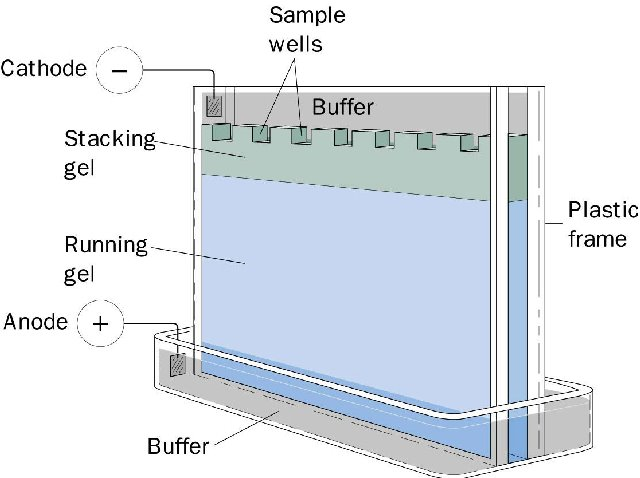
\includegraphics[width=0.4\textwidth]{SDS-PAGE.jpg}
		\end{figure} 
	
	\subsection{\label{sec:TinMet}Tinción con Azul de Coomasie}
	
	
\section{\label{sec:Resul}Resultados}


\section{\label{sec:Dis}Discusión de Resultados}


\bibliographystyle{apalike}
\bibliography{proteinasBib}
\end{document}
%
% ****** End of file apssamp.tex ******
